\documentclass{article} % For LaTeX2e
\usepackage{iclr2022_conference,times}
% Optional math commands from https://github.com/goodfeli/dlbook_notation.
%%%%% NEW MATH DEFINITIONS %%%%%

\usepackage{amsmath,amsfonts,bm}

% Mark sections of captions for referring to divisions of figures
\newcommand{\figleft}{{\em (Left)}}
\newcommand{\figcenter}{{\em (Center)}}
\newcommand{\figright}{{\em (Right)}}
\newcommand{\figtop}{{\em (Top)}}
\newcommand{\figbottom}{{\em (Bottom)}}
\newcommand{\captiona}{{\em (a)}}
\newcommand{\captionb}{{\em (b)}}
\newcommand{\captionc}{{\em (c)}}
\newcommand{\captiond}{{\em (d)}}

% Highlight a newly defined term
\newcommand{\newterm}[1]{{\bf #1}}


% Figure reference, lower-case.
\def\figref#1{figure~\ref{#1}}
% Figure reference, capital. For start of sentence
\def\Figref#1{Figure~\ref{#1}}
\def\twofigref#1#2{figures \ref{#1} and \ref{#2}}
\def\quadfigref#1#2#3#4{figures \ref{#1}, \ref{#2}, \ref{#3} and \ref{#4}}
% Section reference, lower-case.
\def\secref#1{section~\ref{#1}}
% Section reference, capital.
\def\Secref#1{Section~\ref{#1}}
% Reference to two sections.
\def\twosecrefs#1#2{sections \ref{#1} and \ref{#2}}
% Reference to three sections.
\def\secrefs#1#2#3{sections \ref{#1}, \ref{#2} and \ref{#3}}
% Reference to an equation, lower-case.
\def\eqref#1{equation~\ref{#1}}
% Reference to an equation, upper case
\def\Eqref#1{Equation~\ref{#1}}
% A raw reference to an equation---avoid using if possible
\def\plaineqref#1{\ref{#1}}
% Reference to a chapter, lower-case.
\def\chapref#1{chapter~\ref{#1}}
% Reference to an equation, upper case.
\def\Chapref#1{Chapter~\ref{#1}}
% Reference to a range of chapters
\def\rangechapref#1#2{chapters\ref{#1}--\ref{#2}}
% Reference to an algorithm, lower-case.
\def\algref#1{algorithm~\ref{#1}}
% Reference to an algorithm, upper case.
\def\Algref#1{Algorithm~\ref{#1}}
\def\twoalgref#1#2{algorithms \ref{#1} and \ref{#2}}
\def\Twoalgref#1#2{Algorithms \ref{#1} and \ref{#2}}
% Reference to a part, lower case
\def\partref#1{part~\ref{#1}}
% Reference to a part, upper case
\def\Partref#1{Part~\ref{#1}}
\def\twopartref#1#2{parts \ref{#1} and \ref{#2}}

\def\ceil#1{\lceil #1 \rceil}
\def\floor#1{\lfloor #1 \rfloor}
\def\1{\bm{1}}
\newcommand{\train}{\mathcal{D}}
\newcommand{\valid}{\mathcal{D_{\mathrm{valid}}}}
\newcommand{\test}{\mathcal{D_{\mathrm{test}}}}

\def\eps{{\epsilon}}


% Random variables
\def\reta{{\textnormal{$\eta$}}}
\def\ra{{\textnormal{a}}}
\def\rb{{\textnormal{b}}}
\def\rc{{\textnormal{c}}}
\def\rd{{\textnormal{d}}}
\def\re{{\textnormal{e}}}
\def\rf{{\textnormal{f}}}
\def\rg{{\textnormal{g}}}
\def\rh{{\textnormal{h}}}
\def\ri{{\textnormal{i}}}
\def\rj{{\textnormal{j}}}
\def\rk{{\textnormal{k}}}
\def\rl{{\textnormal{l}}}
% rm is already a command, just don't name any random variables m
\def\rn{{\textnormal{n}}}
\def\ro{{\textnormal{o}}}
\def\rp{{\textnormal{p}}}
\def\rq{{\textnormal{q}}}
\def\rr{{\textnormal{r}}}
\def\rs{{\textnormal{s}}}
\def\rt{{\textnormal{t}}}
\def\ru{{\textnormal{u}}}
\def\rv{{\textnormal{v}}}
\def\rw{{\textnormal{w}}}
\def\rx{{\textnormal{x}}}
\def\ry{{\textnormal{y}}}
\def\rz{{\textnormal{z}}}

% Random vectors
\def\rvepsilon{{\mathbf{\epsilon}}}
\def\rvtheta{{\mathbf{\theta}}}
\def\rva{{\mathbf{a}}}
\def\rvb{{\mathbf{b}}}
\def\rvc{{\mathbf{c}}}
\def\rvd{{\mathbf{d}}}
\def\rve{{\mathbf{e}}}
\def\rvf{{\mathbf{f}}}
\def\rvg{{\mathbf{g}}}
\def\rvh{{\mathbf{h}}}
\def\rvu{{\mathbf{i}}}
\def\rvj{{\mathbf{j}}}
\def\rvk{{\mathbf{k}}}
\def\rvl{{\mathbf{l}}}
\def\rvm{{\mathbf{m}}}
\def\rvn{{\mathbf{n}}}
\def\rvo{{\mathbf{o}}}
\def\rvp{{\mathbf{p}}}
\def\rvq{{\mathbf{q}}}
\def\rvr{{\mathbf{r}}}
\def\rvs{{\mathbf{s}}}
\def\rvt{{\mathbf{t}}}
\def\rvu{{\mathbf{u}}}
\def\rvv{{\mathbf{v}}}
\def\rvw{{\mathbf{w}}}
\def\rvx{{\mathbf{x}}}
\def\rvy{{\mathbf{y}}}
\def\rvz{{\mathbf{z}}}

% Elements of random vectors
\def\erva{{\textnormal{a}}}
\def\ervb{{\textnormal{b}}}
\def\ervc{{\textnormal{c}}}
\def\ervd{{\textnormal{d}}}
\def\erve{{\textnormal{e}}}
\def\ervf{{\textnormal{f}}}
\def\ervg{{\textnormal{g}}}
\def\ervh{{\textnormal{h}}}
\def\ervi{{\textnormal{i}}}
\def\ervj{{\textnormal{j}}}
\def\ervk{{\textnormal{k}}}
\def\ervl{{\textnormal{l}}}
\def\ervm{{\textnormal{m}}}
\def\ervn{{\textnormal{n}}}
\def\ervo{{\textnormal{o}}}
\def\ervp{{\textnormal{p}}}
\def\ervq{{\textnormal{q}}}
\def\ervr{{\textnormal{r}}}
\def\ervs{{\textnormal{s}}}
\def\ervt{{\textnormal{t}}}
\def\ervu{{\textnormal{u}}}
\def\ervv{{\textnormal{v}}}
\def\ervw{{\textnormal{w}}}
\def\ervx{{\textnormal{x}}}
\def\ervy{{\textnormal{y}}}
\def\ervz{{\textnormal{z}}}

% Random matrices
\def\rmA{{\mathbf{A}}}
\def\rmB{{\mathbf{B}}}
\def\rmC{{\mathbf{C}}}
\def\rmD{{\mathbf{D}}}
\def\rmE{{\mathbf{E}}}
\def\rmF{{\mathbf{F}}}
\def\rmG{{\mathbf{G}}}
\def\rmH{{\mathbf{H}}}
\def\rmI{{\mathbf{I}}}
\def\rmJ{{\mathbf{J}}}
\def\rmK{{\mathbf{K}}}
\def\rmL{{\mathbf{L}}}
\def\rmM{{\mathbf{M}}}
\def\rmN{{\mathbf{N}}}
\def\rmO{{\mathbf{O}}}
\def\rmP{{\mathbf{P}}}
\def\rmQ{{\mathbf{Q}}}
\def\rmR{{\mathbf{R}}}
\def\rmS{{\mathbf{S}}}
\def\rmT{{\mathbf{T}}}
\def\rmU{{\mathbf{U}}}
\def\rmV{{\mathbf{V}}}
\def\rmW{{\mathbf{W}}}
\def\rmX{{\mathbf{X}}}
\def\rmY{{\mathbf{Y}}}
\def\rmZ{{\mathbf{Z}}}

% Elements of random matrices
\def\ermA{{\textnormal{A}}}
\def\ermB{{\textnormal{B}}}
\def\ermC{{\textnormal{C}}}
\def\ermD{{\textnormal{D}}}
\def\ermE{{\textnormal{E}}}
\def\ermF{{\textnormal{F}}}
\def\ermG{{\textnormal{G}}}
\def\ermH{{\textnormal{H}}}
\def\ermI{{\textnormal{I}}}
\def\ermJ{{\textnormal{J}}}
\def\ermK{{\textnormal{K}}}
\def\ermL{{\textnormal{L}}}
\def\ermM{{\textnormal{M}}}
\def\ermN{{\textnormal{N}}}
\def\ermO{{\textnormal{O}}}
\def\ermP{{\textnormal{P}}}
\def\ermQ{{\textnormal{Q}}}
\def\ermR{{\textnormal{R}}}
\def\ermS{{\textnormal{S}}}
\def\ermT{{\textnormal{T}}}
\def\ermU{{\textnormal{U}}}
\def\ermV{{\textnormal{V}}}
\def\ermW{{\textnormal{W}}}
\def\ermX{{\textnormal{X}}}
\def\ermY{{\textnormal{Y}}}
\def\ermZ{{\textnormal{Z}}}

% Vectors
\def\vzero{{\bm{0}}}
\def\vone{{\bm{1}}}
\def\vmu{{\bm{\mu}}}
\def\vtheta{{\bm{\theta}}}
\def\va{{\bm{a}}}
\def\vb{{\bm{b}}}
\def\vc{{\bm{c}}}
\def\vd{{\bm{d}}}
\def\ve{{\bm{e}}}
\def\vf{{\bm{f}}}
\def\vg{{\bm{g}}}
\def\vh{{\bm{h}}}
\def\vi{{\bm{i}}}
\def\vj{{\bm{j}}}
\def\vk{{\bm{k}}}
\def\vl{{\bm{l}}}
\def\vm{{\bm{m}}}
\def\vn{{\bm{n}}}
\def\vo{{\bm{o}}}
\def\vp{{\bm{p}}}
\def\vq{{\bm{q}}}
\def\vr{{\bm{r}}}
\def\vs{{\bm{s}}}
\def\vt{{\bm{t}}}
\def\vu{{\bm{u}}}
\def\vv{{\bm{v}}}
\def\vw{{\bm{w}}}
\def\vx{{\bm{x}}}
\def\vy{{\bm{y}}}
\def\vz{{\bm{z}}}

% Elements of vectors
\def\evalpha{{\alpha}}
\def\evbeta{{\beta}}
\def\evepsilon{{\epsilon}}
\def\evlambda{{\lambda}}
\def\evomega{{\omega}}
\def\evmu{{\mu}}
\def\evpsi{{\psi}}
\def\evsigma{{\sigma}}
\def\evtheta{{\theta}}
\def\eva{{a}}
\def\evb{{b}}
\def\evc{{c}}
\def\evd{{d}}
\def\eve{{e}}
\def\evf{{f}}
\def\evg{{g}}
\def\evh{{h}}
\def\evi{{i}}
\def\evj{{j}}
\def\evk{{k}}
\def\evl{{l}}
\def\evm{{m}}
\def\evn{{n}}
\def\evo{{o}}
\def\evp{{p}}
\def\evq{{q}}
\def\evr{{r}}
\def\evs{{s}}
\def\evt{{t}}
\def\evu{{u}}
\def\evv{{v}}
\def\evw{{w}}
\def\evx{{x}}
\def\evy{{y}}
\def\evz{{z}}

% Matrix
\def\mA{{\bm{A}}}
\def\mB{{\bm{B}}}
\def\mC{{\bm{C}}}
\def\mD{{\bm{D}}}
\def\mE{{\bm{E}}}
\def\mF{{\bm{F}}}
\def\mG{{\bm{G}}}
\def\mH{{\bm{H}}}
\def\mI{{\bm{I}}}
\def\mJ{{\bm{J}}}
\def\mK{{\bm{K}}}
\def\mL{{\bm{L}}}
\def\mM{{\bm{M}}}
\def\mN{{\bm{N}}}
\def\mO{{\bm{O}}}
\def\mP{{\bm{P}}}
\def\mQ{{\bm{Q}}}
\def\mR{{\bm{R}}}
\def\mS{{\bm{S}}}
\def\mT{{\bm{T}}}
\def\mU{{\bm{U}}}
\def\mV{{\bm{V}}}
\def\mW{{\bm{W}}}
\def\mX{{\bm{X}}}
\def\mY{{\bm{Y}}}
\def\mZ{{\bm{Z}}}
\def\mBeta{{\bm{\beta}}}
\def\mPhi{{\bm{\Phi}}}
\def\mLambda{{\bm{\Lambda}}}
\def\mSigma{{\bm{\Sigma}}}

% Tensor
\DeclareMathAlphabet{\mathsfit}{\encodingdefault}{\sfdefault}{m}{sl}
\SetMathAlphabet{\mathsfit}{bold}{\encodingdefault}{\sfdefault}{bx}{n}
\newcommand{\tens}[1]{\bm{\mathsfit{#1}}}
\def\tA{{\tens{A}}}
\def\tB{{\tens{B}}}
\def\tC{{\tens{C}}}
\def\tD{{\tens{D}}}
\def\tE{{\tens{E}}}
\def\tF{{\tens{F}}}
\def\tG{{\tens{G}}}
\def\tH{{\tens{H}}}
\def\tI{{\tens{I}}}
\def\tJ{{\tens{J}}}
\def\tK{{\tens{K}}}
\def\tL{{\tens{L}}}
\def\tM{{\tens{M}}}
\def\tN{{\tens{N}}}
\def\tO{{\tens{O}}}
\def\tP{{\tens{P}}}
\def\tQ{{\tens{Q}}}
\def\tR{{\tens{R}}}
\def\tS{{\tens{S}}}
\def\tT{{\tens{T}}}
\def\tU{{\tens{U}}}
\def\tV{{\tens{V}}}
\def\tW{{\tens{W}}}
\def\tX{{\tens{X}}}
\def\tY{{\tens{Y}}}
\def\tZ{{\tens{Z}}}


% Graph
\def\gA{{\mathcal{A}}}
\def\gB{{\mathcal{B}}}
\def\gC{{\mathcal{C}}}
\def\gD{{\mathcal{D}}}
\def\gE{{\mathcal{E}}}
\def\gF{{\mathcal{F}}}
\def\gG{{\mathcal{G}}}
\def\gH{{\mathcal{H}}}
\def\gI{{\mathcal{I}}}
\def\gJ{{\mathcal{J}}}
\def\gK{{\mathcal{K}}}
\def\gL{{\mathcal{L}}}
\def\gM{{\mathcal{M}}}
\def\gN{{\mathcal{N}}}
\def\gO{{\mathcal{O}}}
\def\gP{{\mathcal{P}}}
\def\gQ{{\mathcal{Q}}}
\def\gR{{\mathcal{R}}}
\def\gS{{\mathcal{S}}}
\def\gT{{\mathcal{T}}}
\def\gU{{\mathcal{U}}}
\def\gV{{\mathcal{V}}}
\def\gW{{\mathcal{W}}}
\def\gX{{\mathcal{X}}}
\def\gY{{\mathcal{Y}}}
\def\gZ{{\mathcal{Z}}}

% Sets
\def\sA{{\mathbb{A}}}
\def\sB{{\mathbb{B}}}
\def\sC{{\mathbb{C}}}
\def\sD{{\mathbb{D}}}
% Don't use a set called E, because this would be the same as our symbol
% for expectation.
\def\sF{{\mathbb{F}}}
\def\sG{{\mathbb{G}}}
\def\sH{{\mathbb{H}}}
\def\sI{{\mathbb{I}}}
\def\sJ{{\mathbb{J}}}
\def\sK{{\mathbb{K}}}
\def\sL{{\mathbb{L}}}
\def\sM{{\mathbb{M}}}
\def\sN{{\mathbb{N}}}
\def\sO{{\mathbb{O}}}
\def\sP{{\mathbb{P}}}
\def\sQ{{\mathbb{Q}}}
\def\sR{{\mathbb{R}}}
\def\sS{{\mathbb{S}}}
\def\sT{{\mathbb{T}}}
\def\sU{{\mathbb{U}}}
\def\sV{{\mathbb{V}}}
\def\sW{{\mathbb{W}}}
\def\sX{{\mathbb{X}}}
\def\sY{{\mathbb{Y}}}
\def\sZ{{\mathbb{Z}}}

% Entries of a matrix
\def\emLambda{{\Lambda}}
\def\emA{{A}}
\def\emB{{B}}
\def\emC{{C}}
\def\emD{{D}}
\def\emE{{E}}
\def\emF{{F}}
\def\emG{{G}}
\def\emH{{H}}
\def\emI{{I}}
\def\emJ{{J}}
\def\emK{{K}}
\def\emL{{L}}
\def\emM{{M}}
\def\emN{{N}}
\def\emO{{O}}
\def\emP{{P}}
\def\emQ{{Q}}
\def\emR{{R}}
\def\emS{{S}}
\def\emT{{T}}
\def\emU{{U}}
\def\emV{{V}}
\def\emW{{W}}
\def\emX{{X}}
\def\emY{{Y}}
\def\emZ{{Z}}
\def\emSigma{{\Sigma}}

% entries of a tensor
% Same font as tensor, without \bm wrapper
\newcommand{\etens}[1]{\mathsfit{#1}}
\def\etLambda{{\etens{\Lambda}}}
\def\etA{{\etens{A}}}
\def\etB{{\etens{B}}}
\def\etC{{\etens{C}}}
\def\etD{{\etens{D}}}
\def\etE{{\etens{E}}}
\def\etF{{\etens{F}}}
\def\etG{{\etens{G}}}
\def\etH{{\etens{H}}}
\def\etI{{\etens{I}}}
\def\etJ{{\etens{J}}}
\def\etK{{\etens{K}}}
\def\etL{{\etens{L}}}
\def\etM{{\etens{M}}}
\def\etN{{\etens{N}}}
\def\etO{{\etens{O}}}
\def\etP{{\etens{P}}}
\def\etQ{{\etens{Q}}}
\def\etR{{\etens{R}}}
\def\etS{{\etens{S}}}
\def\etT{{\etens{T}}}
\def\etU{{\etens{U}}}
\def\etV{{\etens{V}}}
\def\etW{{\etens{W}}}
\def\etX{{\etens{X}}}
\def\etY{{\etens{Y}}}
\def\etZ{{\etens{Z}}}

% The true underlying data generating distribution
\newcommand{\pdata}{p_{\rm{data}}}
% The empirical distribution defined by the training set
\newcommand{\ptrain}{\hat{p}_{\rm{data}}}
\newcommand{\Ptrain}{\hat{P}_{\rm{data}}}
% The model distribution
\newcommand{\pmodel}{p_{\rm{model}}}
\newcommand{\Pmodel}{P_{\rm{model}}}
\newcommand{\ptildemodel}{\tilde{p}_{\rm{model}}}
% Stochastic autoencoder distributions
\newcommand{\pencode}{p_{\rm{encoder}}}
\newcommand{\pdecode}{p_{\rm{decoder}}}
\newcommand{\precons}{p_{\rm{reconstruct}}}

\newcommand{\laplace}{\mathrm{Laplace}} % Laplace distribution

\newcommand{\E}{\mathbb{E}}
\newcommand{\Ls}{\mathcal{L}}
\newcommand{\R}{\mathbb{R}}
\newcommand{\emp}{\tilde{p}}
\newcommand{\lr}{\alpha}
\newcommand{\reg}{\lambda}
\newcommand{\rect}{\mathrm{rectifier}}
\newcommand{\softmax}{\mathrm{softmax}}
\newcommand{\sigmoid}{\sigma}
\newcommand{\softplus}{\zeta}
\newcommand{\KL}{D_{\mathrm{KL}}}
\newcommand{\Var}{\mathrm{Var}}
\newcommand{\standarderror}{\mathrm{SE}}
\newcommand{\Cov}{\mathrm{Cov}}
% Wolfram Mathworld says $L^2$ is for function spaces and $\ell^2$ is for vectors
% But then they seem to use $L^2$ for vectors throughout the site, and so does
% wikipedia.
\newcommand{\normlzero}{L^0}
\newcommand{\normlone}{L^1}
\newcommand{\normltwo}{L^2}
\newcommand{\normlp}{L^p}
\newcommand{\normmax}{L^\infty}

\newcommand{\parents}{Pa} % See usage in notation.tex. Chosen to match Daphne's book.

\DeclareMathOperator*{\argmax}{arg\,max}
\DeclareMathOperator*{\argmin}{arg\,min}

\DeclareMathOperator{\sign}{sign}
\DeclareMathOperator{\Tr}{Tr}
\let\ab\allowbreak


%######## APS360: Uncomment your submission name
\newcommand{\apsname}{Project Proposal}
%\newcommand{\apsname}{Progress Report}
%\newcommand{\apsname}{Final Report}

%######## APS360: Put your Group Number here
\newcommand{\gpnumber}{4}

\usepackage{hyperref}
\usepackage{url}
\usepackage{graphicx}
\usepackage{float}
\restylefloat{table}

%######## APS360: Put your project Title here
\title{Autonomous Car using Deep Learning Project Proposal\\}


%######## APS360: Put your names, student IDs and Emails here
\author{Rudra Dey  \\
Student\# 1010124866\\
\texttt{rudra.dey@mail.utoronto.ca } \\
\And
Pravin Kalaivannan  \\
Student\# 1010141295 \\
\texttt{pravin.kalaivannan@mail.utoronto.ca} \\
\AND
Aadavan Vasudevan  \\
Student\# 1010101514 \\
\texttt{aadavan.vasudevan@mail.utoronto.ca} \\
\And
Abishan Baheerathan \\
Student\# 1010218756 \\
\texttt{abishan.baheerathan@mail.utoronto.ca} \\
\AND
}

% The \author macro works with any number of authors. There are two commands
% used to separate the names and addresses of multiple authors: \And and \AND.
%
% Using \And between authors leaves it to \LaTeX{} to determine where to break
% the lines. Using \AND forces a linebreak at that point. So, if \LaTeX{}
% puts 3 of 4 authors names on the first line, and the last on the second
% line, try using \AND instead of \And before the third author name.

\newcommand{\fix}{\marginpar{FIX}}
\newcommand{\new}{\marginpar{NEW}}

\iclrfinalcopy 
%######## APS360: Document starts here
\begin{document}

\maketitle

\begin{abstract}
This document presents our team's approach to developing an autonomous car system. This document contains research done on similar projects, data processing methods, 
architecture details, and a baseline comparison model. Our team looked into ethical 
concerns and potential major risks that could occur with this project. Further, the team came 
together to form a detailed project plan. This plan contains important tasks, 
who is responsible for each task, and project deadlines.\\
%######## APS360: Do not change the next line. This shows your Main body page count.
Total Pages: \pageref{last_page}
\end{abstract}



\section{Introduction}


This project proposal will discuss our team’s plan to train an 
autonomous car. The motivation behind this project comes from a shared interest in robotics and deep 
learning among the team. Our team’s goal is to train the car to drive itself using cameras and control 
input. This project will be using a CNN model, public datasets such as the Udacity self-driving car dataset, 
and custom data that is collected through a mounted camera on an RC car. This is an interesting project 
because we get to explore the world of autonomous vehicles and the only sensor we plan on using is a camera. 
This project needs deep learning to process data in a fast and reliable way. We need to code procedural 
instructions for different situations based on our sensor (the camera), but this seems dangerous as humans 
can not think of every possible situation. A training model can handle this problem in a generalized way 
which is what we need to accomplish our goal. 
 



\section{Background and Related Works}
\label{headings}

\subsection{Autonomous Car Related Projects}

Through the use of deep learning, many autonomous car projects have been developed and tested, showing the potential of this technology in real-world applications. 
The following is an overview of five works related to autonomous vehicles using deep learning.  


\subsubsection{Deep CNN End-to-End Learning for Autonomous RC Cars \citep{bhutta2023deep}}

 
In this study, end-to-end learning using deep convolutional neural networks (CNNs) was used to autonomously control an RC car around a race track. 
A front-facing camera is used to collect images of the car’s view, which is fed to the model. The CNN extracts features through convolutional and pooling layers, 
then applies the nonlinear ReLU activation function, which is then passed through 3 fully connected layers to generate the output of necessary steering angles 
and speed the car needs to travel \citep{bhutta2023deep}.

\subsubsection{Autonomous RC Car Using Neural Networks \citep{Mallik2023}}

This project explores autonomous driving through a small RC car using a Raspberry Pi and a CNN based end-to-end steering angle prediction system. 
To train the model, the car was manually driven around a track and the Raspberry Pi was used to track the analog steering inputs along with recording video frames 
taken at 10-20 fps. The project highlights limited computing resources from the Pi’s onboard chips which may constrain CNN complexity along with data 
diversity being an issue where overfitting to a single environment leads to issues in other environments. Additionally, the project highlights the 
feasibility of deep learning for autonomous navigation and that it can be scaled up to larger robotic systems.

\subsubsection{Development of Single-board Computer-based Self-Driving Car Model \citep{9751873}}

In this paper, an RC car based on the DonkeyCar project, powered by a Nvidia Jetson Nano and controlled by a CNN was used to drive autonomously around a track. The
CNN uses live photos of the car’s front view to predict the steering angle and speed required. The authors created varied training set sizes of 
3000, 6000, 12000 and 24000 along with variations of network depth of between two and five layers of convolutional layers to find the best model \citep{9751873}. 
Their results showed that the model with 24000 images with three convolution layers performed the best with an absolute error at 0.18257 \citep{9751873}. 
Additionally, the results showed that having more data consistently reduced error, while adding layers above three had diminishing returns. 


\subsubsection{CNN based End to End Learning Steering Angle Prediction for Autonomous Electric Vehicles \citep{Mygapula2021}}

This paper explores CNN based end-to-end learning for steering angle prediction in autonomous vehicles using images captured of the front 
view of the car which is passed through to the model in a Jetson TX1. The team trained 3 different models based on different CNN architectures 
with different numbers of layers and the results showed that the CNN model with 4 CNN layers and 4 connected layers performed the 
best with 0.0354 test loss \citep{Mygapula2021}. These results highlight the viability of CNNs in learning steering behaviours compared to typical 
approaches in which systems are broken into multiple stages (such as road and object detection, and path planning)as it has fewer potential failure points.

\subsubsection{End to End Learning for Self-Driving Cars \citep{bojarski2016endendlearningselfdriving}}

In this paper, the team trained a CNN to map raw pixels from a front-facing camera directly to steering commands for a car. 
The network made up of nine layers, with one normalization layer, five convolutional layers and three fully connected layers 
was trained to minimize the mean squared error between steering commands and the human driver’s inputs. Using only 
72 hours of driving data, the team was able to successfully train the car to operate in diverse conditions showing 
how a CNN can perform the entire task without manual decomposition into smaller systems \citep{bojarski2016endendlearningselfdriving}. 

\section{Data Processing}
\label{headings}


The Data Processing pipeline for the self-driving car project has three critical phases:
Data Collection, Data Cleaning and Preprocessing, and Dataset Splitting. These phases are
needed to ensure proper and high-quality training, validation, and testing of our model.

\subsection{Data Collection}

\subsubsection{Public Datasets}
\begin{itemize}
  \item Udacity Self-Driving Car Dataset \citep{udacity_self_driving_car_2021}
  \item Berkeley DeepDrive (BDD100K) \citep{bdd100k_2018}
\end{itemize}

\subsubsection{Custom Data Collection}
\begin{itemize}
  \item Simulated Data: Using CARLA Simulator to generate high-resolution images with corresponding control commands \citep{Dosovitskiy17}
  \item Real-World Data: Dash-mounted Camera on RC Cars.
\end{itemize}


\subsection{Data Cleaning and Preprocessing}

This phase involves preparing the image data and labels to maximize model accuracy. 
This includes image normalization and label consistency checks.

\subsubsection{Remove Corrupted or Blurry Frames}
Removal of incomplete metadata, heavy blur, overexposure, and distorted images using automated filters.
These filters include: Laplacian Variance for blur detection, Histogram Analysis for overexposure, 
and Pixel Clipping Detection.


\subsubsection{Image Resizing and Normalization}
All images are resized to a uniform size of 320x240 pixels to match input expectations for deep CNNs. Additionally, 
pixel values are normalized to seed up convergence during training.

\subsubsection{Label Alignment and Verification}
Control labels are synchronized with their corresponding images using timestamps. Outliers and inconsistent 
data are flagged and removed. 

\subsection{Dataset Splitting}
The dataset is split into:
\begin{itemize}
  \item 80\% Training
  \item 10\% Validation 
  \item 10\% Testing 
\end{itemize}

Since we are using data that comes from continuous streams, randomly shuffling data could have
it so very similar frames of the stream can land in training, validation, and testing leading to 
memorization of the data. Thus, we will split the data chronologically, first 80\% goes to 
training, the next 10\% goes to validation, and the last 10\% goes to testing. This way the test set 
includes unseen time segments from the drive. 


\section{Architecture}

The neural network architecture is designed to take images of size 320x240x3 (height, width, RGB) of the
front-facing camera on the dash or hood of the car. With this, the neural network outputs/predictions are the 
continuous steering angle values for the car (regression task). Using multiple Conv2d layers, with 5x5 kernels, 
a stride of 1, and a ReLU activation to introduce non-linearity we aim to extract spatial features, like 
lane lines, edges, and road curvature. These feature maps are passed through a flattened layer and then into 
a fully connected layer which allows the model to learn high-level representations. The final output layer is a single neuron
with a linear activation function capturing the steering angle of the car. This implies that the speed of the car
is constant from the start, or could be controlled manually.

\subsection{Normalization}
To improve generalization we:
\begin{itemize}
  \item Batch normalization is applied after convolutional layers to normalize activations.
  \item L2 Weight Decay is applied during optimization to penalize overly complex models which leads to overfitting.
\end{itemize}

\subsection{Training Method}
This network is trained as a regression problem, where the goal is to minimize the error between predicted and actual
steering angles. We will use the following to train our model:
\begin{itemize}
  \item Loss Function: Using Mean Squared Error (MSE) to calculate the loss, penalizing large changes in steering
  predictions.
  \item Optimizer: Using the Adam Optimizer we will update network eights during training with adaptivative learning rates.
  \item Training Metrics: Root Mean Squared Error (RMSE) and Mean Absolute Error (MAE) are used to evaluate the accuracy of steering predictions.
\end{itemize}



\section{Citations, figures, tables, references}
\label{others}

These instructions apply to everyone, regardless of the format being used.

\subsection{Citations within the text}

Citations within the text should be based on the \texttt{natbib} package
and include the authors' last names and years (with the ``et~al.'' construct
for more than two authors). When the authors or the publication are
included in the sentence, the citation should not be in parenthesis using \verb|\citet{}| (as
in ``See \citet{Hinton06} for more information.''). Otherwise, the citation
should be in parenthesis using \verb|\citep{}| (as in ``Deep learning shows promise to make progress
towards AI~\citep{Bengio+chapter2007}.'').

The corresponding references are to be listed in alphabetical order of
authors, in the \textsc{References} section. As to the format of the
references themselves, any style is acceptable as long as it is used
consistently.

To cite a new paper, first, you need to add that paper's BibTeX information to \verb+APS360_ref.bib+ file and then you can use the \verb|\citep{}| command to cite that in your main document. 

\subsection{Footnotes}

Indicate footnotes with a number\footnote{Sample of the first footnote} in the
text. Place the footnotes at the bottom of the page on which they appear.
Precede the footnote with a horizontal rule of 2~inches
(12~picas).\footnote{Sample of the second footnote}

\subsection{Figures}

All artwork must be neat, clean, and legible. Lines should be dark
enough for purposes of reproduction; art work should not be
hand-drawn. The figure number and caption always appear after the
figure. Place one line space before the figure caption, and one line
space after the figure. The figure caption is lower case (except for
first word and proper nouns); figures are numbered consecutively.

Make sure the figure caption does not get separated from the figure.
Leave sufficient space to avoid splitting the figure and figure caption.

You may use color figures.
However, it is best for the
figure captions and the paper body to make sense if the paper is printed
either in black/white or in color.

\begin{figure}[h]
\begin{center}
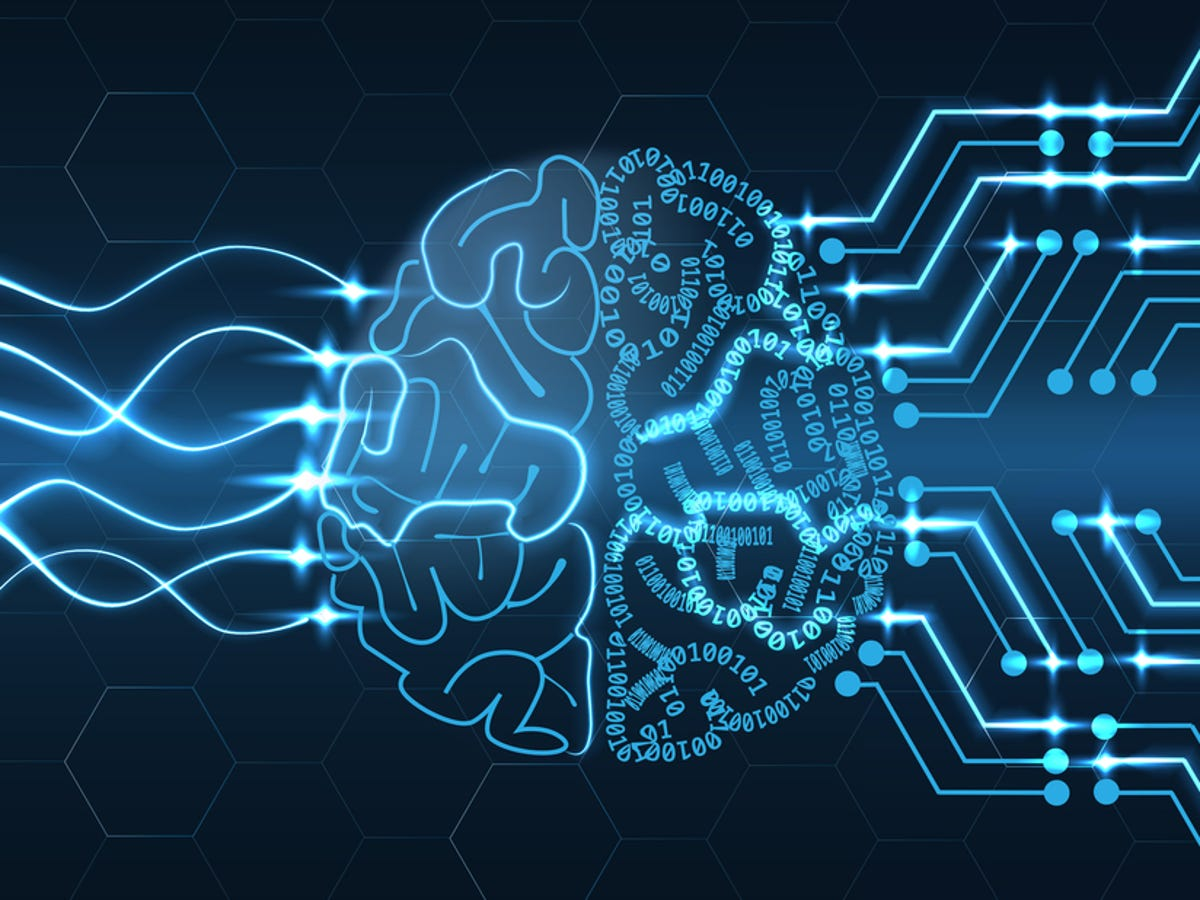
\includegraphics[width=0.6\textwidth]{Figs/td-deep-learning.jpg}
\end{center}
\caption{Sample figure caption. Image: ZDNet}
\end{figure}

\subsection{Tables}

All tables must be centered, neat, clean and legible. Do not use hand-drawn
tables. The table number and title always appear before the table. See
Table~\ref{sample-table}.

Place one line space before the table title, one line space after the table
title, and one line space after the table. The table title must be lower case
(except for first word and proper nouns); tables are numbered consecutively.

\begin{table}[t]
\caption{Sample table title}
\label{sample-table}
\begin{center}
\begin{tabular}{ll}
\multicolumn{1}{c}{\bf PART}  &\multicolumn{1}{c}{\bf DESCRIPTION}
\\ \hline \\
Dendrite         &Input terminal \\
Axon             &Output terminal \\
Soma             &Cell body (contains cell nucleus) \\
\end{tabular}
\end{center}
\end{table}



\section{Baseline Model}

A hand-coded rule-based controller serves as a reasonable baseline for evaluating the performance of the autonomous car. 
This baseline model simulates traditional line-following logic, where decisions are made using simple heuristics based on 
pixel colour thresholds and pre-defined turning logic \citep{LIKMETA2020103568}. The rule-based controller follows a deterministic flow, first, the incoming 
video frame is converted to grayscale or HSV colour space, and then a threshold is applied to detect the track line (usually a black line 
on a white surface or vice versa) \citep{LIKMETA2020103568}. The centroid of the detected line is computed, and based on its position relative to the image center, 
turning decisions are made. For example, steering left if the line is on the left half of the image, right if on the right half, and forward if 
centered \citep{bojarski2016endendlearningselfdriving}. This model does not involve learning or generalization; it is purely reactive and works well in constrained, consistent environments 
with high-contrast tracks. While simplistic, this approach is widely used as a baseline in autonomous driving projects due to its reproducibility 
and interpretability.

\section{Ethical Considerations}

\subsection{Model Usage}
Since this project involves physical hardware operating in real time, safety is a primary concern. The model may make poor decisions in edge cases 
(obstacles, unfamiliar lighting conditions), which could lead to hardware damage or unintended collisions \citep{dalrymple2024guaranteedsafeaiframework}. If used as part of a demonstration 
involving human interaction, ensuring safety measures (kill switches, limited speed) is essential. Another ethical concern is over-reliance on the 
model's predictions. If used in future deployments (real vehicles or educational kits), assuming the trained model can handle all situations without 
proper validation may mislead users and cause harm or accidents \citep{laskey2017comparinghumancentricrobotcentricsampling}. 


\subsection{Data Collection}
The data used for imitation learning is sourced from human demonstrations. A bias may arise if only a single driving style or track layout is captured.
For instance, if the human driver consistently takes tight turns or drives aggressively, the model may learn to imitate that behaviour, limiting 
generalization to new tracks or drivers. Additionally, reinforcement learning episodes are generated in a simulated or controlled environment 
\citep{laskey2017comparinghumancentricrobotcentricsampling}. 
This might restrict the model's robustness in diverse real-world settings. Ethical considerations also include ensuring no unnecessary wear is inflicted 
on hardware during data collection or that any modifications to the car setup are clearly documented and standardized.

\section{Project Plan}
To ensure the seamless progression of the project and collaboration among team members, we have devised guidelines and a timeline as seen below.

\subsection{Team Guidelines}

\begin{table}[H]
\caption{Meeting Specifications}
\begin{center}
\begin{tabular}{|l|l|}
\hline
\textbf{Meeting Guidelines} & \textbf{Details} \\ \hline
In-person meeting           & Location and time decided by the team \\ \hline
Online meetings             & Tuesdays (3-5 pm) and Saturdays (1-3 pm) \\ \hline
Absence Notification        & Must notify team 24 hours before the meeting if they will be absent \\ \hline
\end{tabular}
\end{center}
\end{table}

\textbf{Communication Guidelines}
\begin{itemize}
  \item Group chat is active on weekdays and weekends (24/7)
  \item Group chat is active on weekdays and weekends (24/7)
  \item Members are required to frequently check discord messages (less than 2 hour response time)
\end{itemize}

\textbf{Collaboration Guidelines}
\begin{itemize}
  \item The team will be working together in a GitHub repository
  \item Each member is required to give a daily update message on their progress
  \item If conflicts arise, the team must discuss them together and decide on a solution that makes everyone happy
  \item Ensure the code has informational comments that help the team understand it
\end{itemize}

\subsection{Project Timeline}



\section{Risk Register}
The risk register contains some scenarios that could negatively impact our project. 
These potential risks negatively affect deadlines, quality of work, and more. Our team has 
discussed these scenarios and come up with solutions for each project risk. 

\begin{table}[H]
\caption{Project Risks}
\centering
\begin{tabular}{|p{4cm}|p{2.5cm}|p{7cm}|}
\hline
\textbf{Project Risk} & \textbf{Likelihood} & \textbf{Solution} \\ \hline
A teammate drops the course & Unlikely & The team has to approach splitting up tasks differently as teammates will now have more responsibilities. We have to start tasks earlier and move internal deadlines to an earlier date because each member has more tasks to complete. \\ \hline
Model training takes longer than expected & Likely & It’s common to procrastinate on less important or easier tasks, so this would be the time to complete them. The team should start working on tasks earlier, so if this does occur it doesn’t affect project deadlines. \\ \hline
Experience hardware problems during testing & Likely & The team should keep extra hardware components in case they fail the during testing stages. Also, try not to overuse the physical components, and use simulation software to test. \\ \hline
The model works in simulation but not on a physical RC car & Likely & We shouldn’t fully rely on simulations and should test the model on the physical RC car frequently. The earlier the team faces these issues, the longer we have to fix them. Compare the results from simulation and physical RC car and that might help solve problems. \\ \hline
If teammate misses an internal deadline & Likely & The team should hold everyone accountable as each member is responsible for their assigned tasks. The teammate should finish tasks as soon as possible after the missed deadline because this will hold back the team. \\ \hline
\end{tabular}
\end{table}


\section{Final instructions}
Do not change any aspects of the formatting parameters in the style files.
In particular, do not modify the width or length of the rectangle the text
should fit into, and do not change font sizes (except perhaps in the
\textsc{References} section; see below). Please note that pages should be
numbered.


\subsubsection*{Author Contributions}
If you'd like to, you may include  a section for author contributions as is done
in many journals. This is optional and at the discretion of the authors.

\subsubsection*{Acknowledgments}
Use unnumbered third level headings for the acknowledgments. All
acknowledgments, including those to funding agencies, go at the end of the paper.

\label{last_page}

\bibliography{APS360_ref}
\bibliographystyle{iclr2022_conference}

\end{document}
